\section{Исследование и построение решения задачи}
\label{sec:Chapter3} \index{Chapter3}
\subsection{Архитектурное решение}

\textbf{В работе реализована стратегия абстрагирования примитивных типов посредством их представления в виде объектов высокоуровневой системы типов, где примитивные операции (арифметика, сравнения) выполняются непосредственно над объектным аналогом примитивного типа. Физическое представление примитивов и низкоуровневые оптимизации генерируются компилятором после этапа семантического анализа, не влияя на корректность и согласованность правил типизации.}

\subsection{Обоснование выбора стратегии}
На основании проведённого обзора существующих решений выбрана стратегия <<Примитивы как оптимизация компилятора>> по следующим причинам:

\begin{enumerate}
    \item \textbf{Упрощение семантического анализа}
    \begin{itemize}[label={--}]
        \item Анализатор работает только с объектными типами (например, \texttt{Int} как класс-обёртка)
        \item Устранение дуализма типов (как в Java) и проблем упаковки (как в C\#)
    \end{itemize}

    \item \textbf{Совместимость с целями языка}
    \begin{itemize}[label={--}]
        \item Чистая объектная модель критична для семантической согласованности высокоуровневого управляемого языка.
    \end{itemize}

    \item \textbf{Практическая эффективность}
    \begin{itemize}[label={--}]
        \item Оптимизации (анбоксинг, инлайнинг методов - подстановка тела непосредственно в место вызова) выполняются на последних этапах и не нарушают семантику проверки типов.
    \end{itemize}
\end{enumerate}

\newpage

\subsection{Описание решения}
\begin{itemize}[leftmargin=*]
    \item Все примитивоподобные типы становятся экземплярами Object
    \item Замена на низкоуровневые примитивы выполняется только на этапе оптимизации компиляции
    \item Именение семантики массивов во время исполнения во избежание неэффективной работы с ними
\end{itemize}

\begin{figure}[h]
\centering
\resizebox{\textwidth}{!}{
\begin{tikzpicture}[
    node distance=1cm,
    stage/.style={rectangle, draw=blue!50, fill=blue!10, thick, minimum width=2cm, minimum height=1cm, align=center},
    arrow/.style={->, >=stealth, thick},
    font=\small
]

\node (lex) [stage] {Лексический\\анализ};
\node (parse) [stage, right=of lex] {Синтаксический\\анализ};
\node (sem) [stage, right=of parse] {Семантический\\анализ};
\node (opt) [stage, right=of sem] {Оптимизация};
\node (codegen) [stage, right=of opt] {Генерация\\кода};

\draw [arrow] (lex) -- (parse);
\draw [arrow] (parse) -- (sem);
\draw [arrow] (sem) -- (opt);
\draw [arrow] (opt) -- (codegen);

\node [below=0.3cm of sem, font=\footnotesize, text width=3cm, align=center] {Работа \\исключительно с \\объектными типами};
\node [above=0.3cm of opt, font=\footnotesize, text width=3cm, align=center] {Замена на\\низкоуровневые\\примитивы};

\end{tikzpicture}
}
\caption{Этапы работы компилятора с выделением семантического анализа}
\label{fig:compiler_pipeline}
\end{figure}

\textbf{Новая унифицированная система типов предусматривает:}
\begin{enumerate}[leftmargin=*]
    \item Каждый примитивный тип полностью эквивалентен своей объектной обёртке, являющейся подклассом Object
    (включая специальные типы: void/Void, undefined/Undefined, null/Null)
    \begin{itemize}[label={--}]
        \item Арифметические операции выполняются непосредственно над объектами без распаковки
        \item Тип объектный примитивоподобный тип становится полноценным участником union-типов
        \item Операторы \code{==} и \code{===} реализуют сравнение по значению (аналогично поведению для String)
    \end{itemize}

\end{enumerate}

\subsection{Изменения в семантике языка}
\subsubsection{Эквивалентные сценарии}
Для наглядности далее в тексте в качестве базового примера будут использоваться типы:
int (примитивный) → Int (объектный аналог)
\begin{figure}[H]
    \centering
    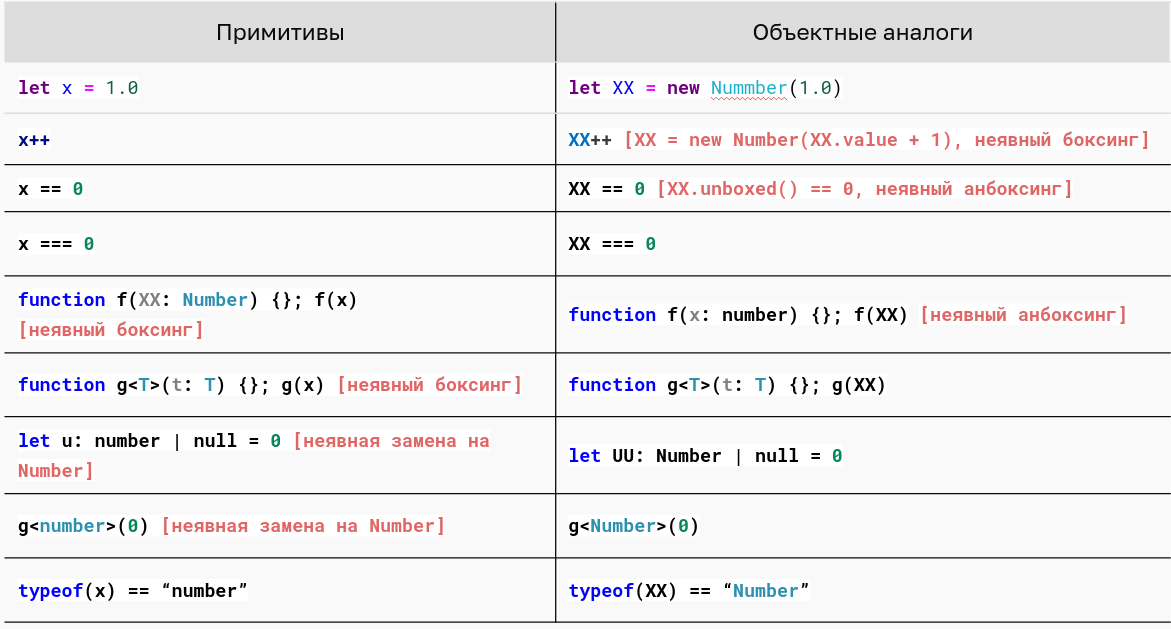
\includegraphics[scale=0.4]{same.png}
    \caption{Выделены места, где ранее выполнялись неявные преобразования}
    \label{fig:example}
\end{figure}

\subsubsection{Новые допустимые конструкции}

\begin{lstlisting}
xx.toStrint() // ошибка компиляции до изменений, будет работать после
xx instanceof Object // ошибка компиляции до изменений, будет работать после
\end{lstlisting}


\subsection{План реализации}
\begin{enumerate}
    \item \textbf{Модификация системы типов}: Убрать примитивные типы на этапе проверки корректности типов в арифметических операциях и преобразованиях типов
    \item \textbf{Обработка констант}: Изменить представление литералов на этапе свёртки констант на объектные типы
    \item \textbf{Оптимизация перед кодогенерацией}: Имплементировать модуль-оптимизацию, где объектные типы будут по возможности заменяться примитивными
\end{enumerate}

\newpage